\documentclass[journal,12pt,twocolumn]{IEEEtran}
%
\usepackage{setspace}
\usepackage{gensymb}
%\doublespacing
\singlespacing

%\usepackage{graphicx}
%\usepackage{amssymb}
%\usepackage{relsize}
\usepackage[cmex10]{amsmath}
%\usepackage{amsthm}
%\interdisplaylinepenalty=2500
%\savesymbol{iint}
%\usepackage{txfonts}
%\restoresymbol{TXF}{iint}
%\usepackage{wasysym}
\usepackage{amsthm}
%\usepackage{iithtlc}
\usepackage{mathrsfs}
\usepackage{txfonts}
\usepackage{stfloats}
\usepackage{bm}
\usepackage{cite}
\usepackage{cases}
\usepackage{subfig}
%\usepackage{xtab}
\usepackage{longtable}
\usepackage{multirow}
%\usepackage{algorithm}
%\usepackage{algpseudocode}
\usepackage{enumitem}
\usepackage{mathtools}
\usepackage{steinmetz}
\usepackage{tikz}
\usepackage{circuitikz}
\usepackage{verbatim}
\usepackage{tfrupee}
\usepackage[breaklinks=true]{hyperref}
%\usepackage{stmaryrd}
\usepackage{tkz-euclide} % loads  TikZ and tkz-base
%\usetkzobj{all}
\usetikzlibrary{calc,math}
\usepackage{listings}
    \usepackage{color}                                            %%
    \usepackage{array}                                            %%
    \usepackage{longtable}                                        %%
    \usepackage{calc}                                             %%
    \usepackage{multirow}                                         %%
    \usepackage{hhline}                                           %%
    \usepackage{ifthen}                                           %%
  %optionally (for landscape tables embedded in another document): %%
    \usepackage{lscape}     
\usepackage{multicol}
\usepackage{chngcntr}
%\usepackage{enumerate}

%\usepackage{wasysym}
%\newcounter{MYtempeqncnt}
\DeclareMathOperator*{\Res}{Res}
%\renewcommand{\baselinestretch}{2}
\renewcommand\thesection{\arabic{section}}
\renewcommand\thesubsection{\thesection.\arabic{subsection}}
\renewcommand\thesubsubsection{\thesubsection.\arabic{subsubsection}}

\renewcommand\thesectiondis{\arabic{section}}
\renewcommand\thesubsectiondis{\thesectiondis.\arabic{subsection}}
\renewcommand\thesubsubsectiondis{\thesubsectiondis.\arabic{subsubsection}}

% correct bad hyphenation here
\hyphenation{op-tical net-works semi-conduc-tor}
\def\inputGnumericTable{}                                 %%

\lstset{
%language=C,
frame=single, 
breaklines=true,
columns=fullflexible
}
%\lstset{
%language=tex,
%frame=single, 
%breaklines=true
%}


\begin{document}
%


\newtheorem{theorem}{Theorem}[section]
\newtheorem{problem}{Problem}
\newtheorem{proposition}{Proposition}[section]
\newtheorem{lemma}{Lemma}[section]
\newtheorem{corollary}[theorem]{Corollary}
\newtheorem{example}{Example}[section]
\newtheorem{definition}[problem]{Definition}
%\newtheorem{thm}{Theorem}[section] 
%\newtheorem{defn}[thm]{Definition}
%\newtheorem{algorithm}{Algorithm}[section]
%\newtheorem{cor}{Corollary}
\newcommand{\BEQA}{\begin{eqnarray}}
\newcommand{\EEQA}{\end{eqnarray}}
\newcommand{\define}{\stackrel{\triangle}{=}}

\bibliographystyle{IEEEtran}
%\bibliographystyle{ieeetr}


\providecommand{\mbf}{\mathbf}
\providecommand{\pr}[1]{\ensuremath{\Pr\left(#1\right)}}
\providecommand{\qfunc}[1]{\ensuremath{Q\left(#1\right)}}
\providecommand{\sbrak}[1]{\ensuremath{{}\left[#1\right]}}
\providecommand{\lsbrak}[1]{\ensuremath{{}\left[#1\right.}}
\providecommand{\rsbrak}[1]{\ensuremath{{}\left.#1\right]}}
\providecommand{\brak}[1]{\ensuremath{\left(#1\right)}}
\providecommand{\lbrak}[1]{\ensuremath{\left(#1\right.}}
\providecommand{\rbrak}[1]{\ensuremath{\left.#1\right)}}
\providecommand{\cbrak}[1]{\ensuremath{\left\{#1\right\}}}
\providecommand{\lcbrak}[1]{\ensuremath{\left\{#1\right.}}
\providecommand{\rcbrak}[1]{\ensuremath{\left.#1\right\}}}
\theoremstyle{remark}
\newtheorem{rem}{Remark}
\newcommand{\sgn}{\mathop{\mathrm{sgn}}}
\providecommand{\abs}[1]{\left\vert#1\right\vert}
\providecommand{\res}[1]{\Res\displaylimits_{#1}} 
\providecommand{\norm}[1]{\left\lVert#1\right\rVert}
%\providecommand{\norm}[1]{\lVert#1\rVert}
\providecommand{\mtx}[1]{\mathbf{#1}}
\providecommand{\mean}[1]{E\left[ #1 \right]}
\providecommand{\fourier}{\overset{\mathcal{F}}{ \rightleftharpoons}}
%\providecommand{\hilbert}{\overset{\mathcal{H}}{ \rightleftharpoons}}
\providecommand{\system}{\overset{\mathcal{H}}{ \longleftrightarrow}}
	%\newcommand{\solution}[2]{\textbf{Solution:}{#1}}
\newcommand{\solution}{\noindent \textbf{Solution: }}
\newcommand{\cosec}{\,\text{cosec}\,}
\providecommand{\dec}[2]{\ensuremath{\overset{#1}{\underset{#2}{\gtrless}}}}
\newcommand{\myvec}[1]{\ensuremath{\begin{pmatrix}#1\end{pmatrix}}}
\newcommand{\mydet}[1]{\ensuremath{\begin{vmatrix}#1\end{vmatrix}}}
%\numberwithin{equation}{section}
\numberwithin{equation}{subsection}
%\numberwithin{problem}{section}
%\numberwithin{definition}{section}
\makeatletter
\@addtoreset{figure}{problem}
\makeatother

\let\StandardTheFigure\thefigure
\let\vec\mathbf
%\renewcommand{\thefigure}{\theproblem.\arabic{figure}}
\renewcommand{\thefigure}{\theproblem}
%\setlist[enumerate,1]{before=\renewcommand\theequation{\theenumi.\arabic{equation}}
%\counterwithin{equation}{enumi}


%\renewcommand{\theequation}{\arabic{subsection}.\arabic{equation}}

\def\putbox#1#2#3{\makebox[0in][l]{\makebox[#1][l]{}\raisebox{\baselineskip}[0in][0in]{\raisebox{#2}[0in][0in]{#3}}}}
     \def\rightbox#1{\makebox[0in][r]{#1}}
     \def\centbox#1{\makebox[0in]{#1}}
     \def\topbox#1{\raisebox{-\baselineskip}[0in][0in]{#1}}
     \def\midbox#1{\raisebox{-0.5\baselineskip}[0in][0in]{#1}}

\vspace{3cm}


\title{Quiz 10}
\author{S Nithish}
% make the title area
\maketitle

\newpage

%\tableofcontents

\bigskip

\renewcommand{\thefigure}{\theenumi}
\renewcommand{\thetable}{\theenumi}
%\renewcommand{\theequation}{\theenumi}


\begin{abstract}
This document contains the solution of the question from NCERT 9th standard chapter 10 exercise 10.5 problem 4
\end{abstract}

%Download all python codes 
%
%\begin{lstlisting}
%svn co https://github.com/JayatiD93/trunk/My_solution_design/codes
%\end{lstlisting}

%Download all and latex-tikz codes from 
%
%\begin{lstlisting}
%svn co https://github.com/gadepall/school/trunk/ncert/geometry/figs
%\end{lstlisting}
%
\section{Exercise 10.4}
\begin{enumerate}
	\item In the below figure $\angle ABC = 69\degree$, $\angle ACB = 31\degree$, find $\angle BDC$
\begin{figure}[ht]
	\centering
	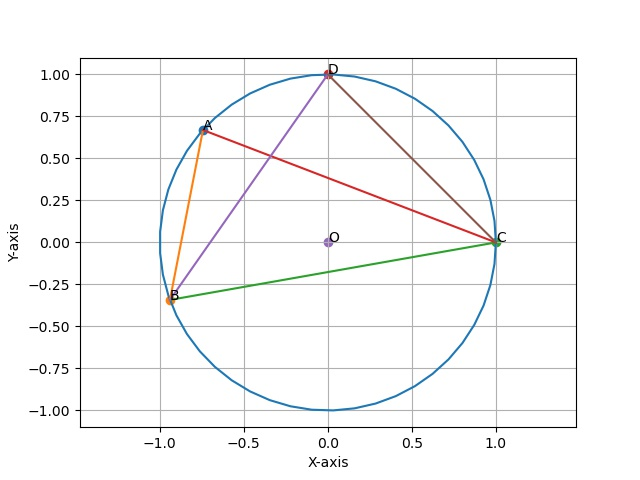
\includegraphics[width = \columnwidth]{figs/plot.jpg}
	\caption{Circle}
	\label{fig:1}
\end{figure}

Let the circle be unit circle centred at origin,

		\begin{align}
			\norm{\vec{x}}^2 = 1
		\end{align}

Let the points A, B, C be such that,

		\begin{align}
			C = \myvec{1\\0}\\
			A = \myvec{\cos \theta_1\\\sin \theta_1}\\
			B = \myvec{\cos \theta_2\\\sin \theta_2}
		\end{align}
		\begin{align}
			BA &= \myvec{\cos \theta_1 - \cos \theta_2\\\sin \theta_1-\sin \theta_2}\\
			BA &= \myvec{-2\sin \brak{\frac{\theta_1-\theta_2}{2}} \sin \brak{\frac{\theta_1+\theta_2}{2}}\\2\cos \brak{\frac{\theta_1+\theta_2}{2}}\sin \brak{\frac{\theta_1-\theta_2}{2}}}\\
			BA &= 2\sin \brak{\frac{\theta_1-\theta_2}{2}}\myvec{-\sin \brak{\frac{\theta_1+\theta_2}{2}}\\\cos \brak{\frac{\theta_1+\theta_2}{2}}}
		\end{align}
		\begin{align}
			BC &= \myvec{1-\cos \theta_2\\-\sin \theta_2}\\
			BC &= \myvec{2\sin^2 \brak{\frac{\theta_2}{2}}\\-2\sin \frac{\theta_2}{2}\cos \frac{\theta_2}{2}}\\
			BC &= 2\sin \frac{\theta_2}{2} \myvec{\sin \frac{\theta_2}{2}\\-\cos \frac{\theta_2}{2}}
		\end{align}
		\begin{align}
			AC &= \myvec{1-\cos \theta_1\\-\sin \theta_1}\\
			AC &= \myvec{2\sin^2 \brak{\frac{\theta_1}{2}}\\-2\sin \frac{\theta_1}{2}\cos \frac{\theta_1}{2}}\\
			AC &= 2\sin \frac{\theta_1}{2} \myvec{\sin \frac{\theta_1}{2}\\-\cos \frac{\theta_1}{2}}
		\end{align}

		\begin{align}
			\angle ABC=69 \degree \\
			\implies \cos 69\degree &= \frac{\vec{BA}^{\top}\vec{BC}}{\norm{\vec{BA}}\norm{\vec{BC}}}\\
												 						 &= -\cos \brak{\frac{\theta_1+\theta_2}{2}-\frac{\theta_2}{2}}\\
						&= -\cos \frac{\theta_1}{2}\\
		    \implies \frac{\theta_1}{2} &= \brak{2k+1}180\degree +69\degree \\
		                       \theta_1 &= \brak{2k+1}360\degree + 138\degree \\
				       \theta_1 &= -360\degree +138\degree \brak{\text{for k=-1}}\\
				  	        &=-222\degree 
		\end{align}

		\begin{align}
			\angle ACB = 31 \degree \\
			\implies \cos 31 \degree &=  \frac{\vec{BC}^{\top}\vec{AC}}{\norm{\vec{BC}}\norm{\vec{AC}}}\\ 
						 &= \myvec{\sin \brak{\frac{\theta_2}{2}}&-\cos \brak{\frac{\theta_2}{2}}}\myvec{\sin \frac{\theta_1}{2} \\ -\cos \frac{\theta_1}{2}}\\
						 &= \cos \brak{\frac{\theta_2-\theta_1}{2}}\\
			\implies \brak{\frac{\theta_2-\theta_1}{2}} &= \brak{k}360\degree +31\degree\\
			       \theta_2-\theta_1 &= \brak{2k}360\degree + 62\degree\\ 
			       \theta_2-\theta_1 &= 62\degree \brak{\text{for k=0}}\\
			       \theta_2+222\degree &= 62\degree\\
			       \theta_2 &= -160\degree 
		\end{align}
		\begin{align}
			A &= \myvec{\cos 222\\ -\sin 222}\\
			B &= \myvec{\cos 160\\ -\sin 160}\\
			C &= \myvec{1\\0}
		\end{align}
		Let us take point D such that,
		\begin{align}
			D = \myvec{0\\1}
		\end{align}
		Then,
		\begin{align}
			DC &= \myvec{1\\0}-\myvec{0\\1} = \myvec{1\\-1}\\
			DB &= \myvec{\cos 160\\ -\sin 160} - \myvec{0\\1}\\
			   &= \myvec{\cos 160\\ -1-\sin 160}\\
			DB &= \myvec{-\sin 70\\ -1-\cos 70} = -2\cos 35 \myvec{\sin 35\\ \cos35}
		\end{align}
	
		\begin{align}
			\cos \angle BDC &= \frac{DC^{\top}DB}{\norm{DC}\norm{DB}}\\
					&= \frac{-2\cos 35 \brak{\sin 35 - \cos 35}}{\brak{2\cos 35}\brak{\sqrt{2}}}\\
					&= \frac{\cos 35 - \sin 35}{\sqrt{2}}\\
					&= \cos \brak{35+45} = \cos 80\\
			\implies \angle DBC = 80 \degree
		\end{align}

\end{enumerate}

%\begin{enumerate}[label=\thesection.\arabic*.,ref=\thesection.\theenumi]
%\num then what are its direction cosines ?berwithin{equation}{enumi}
%\item Verification of the above problem using python code.\\
%%\solution The  following Python code generates Fig. \ref{fig:point_distance}
%%\begin{lstlisting}
%%codes/det_check.py
%%\end{lstlisting}
%
%\end{enumerate}

\end{document}

